% frustum figure (Shaanxi 2008 liberal q19), D midpoint of BC
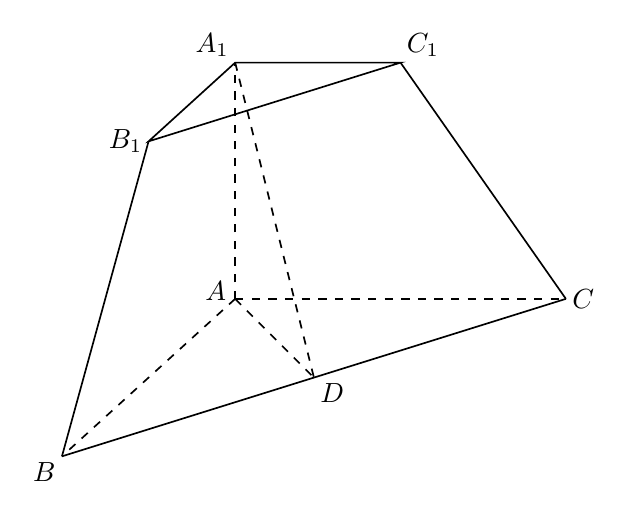
\begin{tikzpicture}[x=1cm,y=1cm,line width=.6pt,font=\normalsize,
  frustum edge/.style={solid,line width=.6pt},
  frustum hidden/.style={dashed,line width=.6pt},
  frustum label/.style={font=\normalsize,inner sep=2pt}]
\coordinate (A) at (0,0);
\coordinate (B) at (-2.2,-2.0);
\coordinate (C) at (4.2,0);
\coordinate (D) at (1.0000000000,-1.0000000000);
\coordinate (A1) at (0,3.0);
\coordinate (B1) at (-1.1000000000,2.0000000000);
\coordinate (C1) at (2.1000000000,3.0000000000);
% solid: bottom BC, laterals, top triangle
\draw[frustum edge] (B)--(D)--(C);
\draw[frustum edge] (B)--(B1);
\draw[frustum edge] (C)--(C1);
\draw[frustum edge] (A1)--(B1)--(C1)--cycle;
% dashed: bottom hidden, vertical, medians
\draw[frustum hidden] (A)--(B);
\draw[frustum hidden] (A)--(C);
\draw[frustum hidden] (A)--(D);
\draw[frustum hidden] (A)--(A1);
\draw[frustum hidden] (A1)--(D);
% labels
\node[frustum label,left,xshift=-1pt,yshift=3pt] at (A) {$A$};
\node[frustum label,below left] at (B) {$B$};
\node[frustum label,right] at (C) {$C$};
\node[frustum label,below right] at (D) {$D$};
\node[frustum label,above left] at (A1) {$A_{1}$};
\node[frustum label,left] at (B1) {$B_{1}$};
\node[frustum label,above right] at (C1) {$C_{1}$};
\end{tikzpicture}
